\section{Definici\'on Formal del Problema}
\label{sec:definition}

Sea $G = (V,E)$ un grafo (dirigido o no), donde $V$ es el conjunto de
nodos y $E$ el conjunto de arcos. Sea $A$ un conjunto de agentes
interesados en alcanzar un punto com\'un $t \in V$. Se tiene
que cada agente $a \in A$, se encuentra en algún nodo del grafo
denotado $pos(a)$. Además, se define para $a$ la función
de costos de su desplazamiento por el grafo
$\lambda_a : E \longrightarrow \mathbb{R}^{\geq 0}$.
Se considera, sin pérdida de generalidad, que $V$ y $E$ son comunes para
todos los agentes, con el fin de no generar inconsistencias en la
información compartida entre estos. Sin embargo, cada agente puede tener
función de costos distintas, adaptadas a sus restricciones.
Sea $path(a)$ con $a \in A$, el camino que está siguiendo el agente
$a$ hasta el nodo $t$.

Previamente, el grado de emboscada (\ref{eq:prev})
efectuado por el conjunto de agentes
$A$ al nodo $t$ se defini\'o como \cite{FGC12e}\cite{FGC12}:

\begin{small}
\begin{eqnarray}
 \Phi(t) &=& 
 \dfrac{|\{ i : path(j) = <pos(j),\ \ldots,\ i,\ t>, j \in A\}|}
	  {\min(|\{ <i,t> : <i,t> \in E \} |,|A|) }
\label{eq:prev}
\end{eqnarray}
\end{small}

Esta m\'etrica define la emboscada como la proporción de nodos adyacentes
al nodo objetivo desde los cuales algún agente está alcanzándolo. Acotando
este valor con res\-pec\-to al m\'aximo n\'umero de nodos adyacentes a $t$ mediante
los cuales, con el n\'umero de agentes disponibles, podr\'ia \'este ser alcanzado.
Por lo tanto, $0 \leq \Phi(t) \leq 1$. Bajo estas condiciones, el objetivo
de un algoritmo de generaci\'on de emboscadas es maximizar el
valor de $\Phi(t)$, dando prioridad a la diversidad de los caminos
considerados por el conjunto de agentes sobre su optimalidad.

En la figura \ref{fig:prev_phi}, se pueden observar en el grafo
superior dos agentes situados en los nodos izquierdos. Los caminos
seleccionados por los agentes hasta el destino $t$ se presentan con
una l\'inea continua, mientras que los arcos no seleccionados se
presentan con una l\'inea segmentada. El n\'umero de nodos adyacentes
al destino es de cuatro, de los cuales, s\'olo dos están siendo
considerados en los caminos de los agentes. Sin embargo, es el m\'aximo
grado de emboscada alcanzable con el n\'umero de agentes implicados.
En el escenario inferior se est\'an utilizando dos agentes para cubrir
una \'unica escapatoria, por lo que la emboscada no es \'optima.

\begin{figure}[htb]
	\begin{center}
		\begin{minipage}[b]{0.9\linewidth}
			\centering
			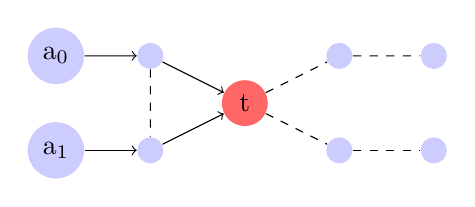
\begin{tikzpicture}
			  [scale=.6,auto=left,every node/.style={circle,fill=blue!20}]
			  \node (n1) at (1,3) {a$_0$};
			  \node (n2) at (3,3) { };
			  
	  		  \node (n3) at (1,1) {a$_1$};
			  \node (n4) at (3,1) { };
			  
			  \node[style={circle,fill=red!60}] (n5) at (5,2) {t};
			  
			  \node (n6) at (7,3) { };
			  \node (n7) at (7,1) { };
			  \node (n8) at (9,3) { };
			  \node (n9) at (9,1) { };
			  		  
			  \foreach \from/\to in {n1/n2,n2/n5,n3/n4,n4/n5}
			  \draw (\from) edge[->] (\to);
	
			  \foreach \from/\to in {n5/n6,n5/n7,n6/n8,n7/n9,n2/n4}
			  \draw (\from) edge[-,dashed] (\to);		  
			\end{tikzpicture}
			
			(a)\\
		\end{minipage}
		
		\bigskip
		\begin{minipage}[b]{0.9\linewidth}
			\centering
			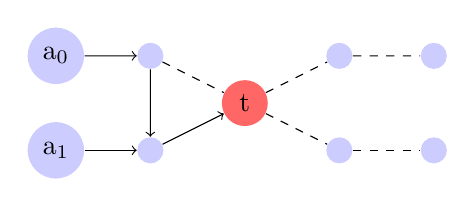
\begin{tikzpicture}
			  [scale=.6,auto=left,every node/.style={circle,fill=blue!20}]
			  \node (n1) at (1,3) {a$_0$};
			  \node (n2) at (3,3) { };
			  
	  		  \node (n3) at (1,1) {a$_1$};
			  \node (n4) at (3,1) { };
			  
			  \node[style={circle,fill=red!60}] (n5) at (5,2) {t};
			  
			  \node (n6) at (7,3) { };
			  \node (n7) at (7,1) { };
			  \node (n8) at (9,3) { };
			  \node (n9) at (9,1) { };
			  		  
			  \foreach \from/\to in {n1/n2,n3/n4,n4/n5,n2/n4}
			  \draw (\from) edge[->] (\to);
	
			  \foreach \from/\to in {n5/n6,n5/n7,n6/n8,n7/n9,n2/n5}
			  \draw (\from) edge[-,dashed] (\to);		  
			\end{tikzpicture}
			
			(b)\\
		\end{minipage}
	\end{center}
	\caption{\label{fig:prev_phi}
	     Ejemplos de emboscadas con dos agentes con valores de $\Phi$ de
	     $1.0$ para (a) dado que cubre dos caminos y $0.5$ para (b) dado que
	     cubre un camino.
	}
\end{figure}

Sin embargo, esta m\'etrica penaliza casos donde no es posible alcanzar
una mejor emboscada, a\'un cuando se cuenta con suficientes agentes, debido
a la configuraci\'on del grafo y a las posiciones iniciales de estos. 
Ejemplos de estos casos pueden ser observados en la figura \ref{fig:error_phi}. En
la situaci\'on superior, se observa que a pesar de contar con cuatro agentes,
las dos salidas restantes no son alcanzables por estos sin pasar antes por el
nodo objetivo. Por otra parte, en la situaci\'on inferior, a pesar de que todas
las salidas son alcanzables por los agentes, no es posible lograr una
configuraci\'on de caminos capaz de cubrir todas las salidas. Para ambos
casos, a pesar de que la asignaci\'on de caminos es la mejor dadas las
condiciones iniciales, la m\'etrica originalmente planteada reporta resultados
sub\'optimos.

\begin{figure}[htb]
	\begin{center}
		\begin{minipage}[b]{0.9\linewidth}
			\centering
			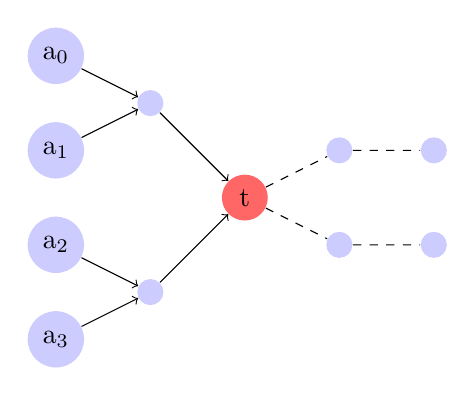
\begin{tikzpicture}
			  [scale=.6,auto=left,every node/.style={circle,fill=blue!20}]
			  \node (n11) at (1,7) {a$_0$};
			  \node (n12) at (1,5) {a$_1$};
			  \node (n2) at (3,6) { };
			  
	  		  \node (n31) at (1,3) {a$_2$};
	  		  \node (n32) at (1,1) {a$_3$};
			  \node (n4) at (3,2) { };
			  
			  \node[style={circle,fill=red!60}] (n5) at (5,4) {t};
			  
			  \node (n6) at (7,5) { };
			  \node (n7) at (7,3) { };
			  \node (n8) at (9,5) { };
			  \node (n9) at (9,3) { };
			  
			  \foreach \from/\to in {n11/n2,n12/n2,n2/n5,n31/n4,n32/n4,n4/n5}
			  \draw (\from) edge[->] (\to);
	
			  \foreach \from/\to in {n5/n6,n5/n7,n6/n8,n7/n9}
			  \draw (\from) edge[-,dashed] (\to);		  
			\end{tikzpicture}
			
			(a)\\
		\end{minipage}
		
		\bigskip
		\begin{minipage}[b]{0.9\linewidth}
			\centering
			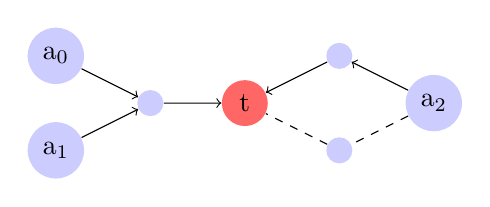
\begin{tikzpicture}
			  [scale=.6,auto=left,every node/.style={circle,fill=blue!20}]
			  \node (n11) at (1,3) {a$_0$};
			  \node (n12) at (1,1) {a$_1$};
			  \node (n2) at (3,2) { };
			  
	  		  \node (n3) at (9,2) {a$_2$};
			  \node (n41) at (7,3) { };
  			  \node (n42) at (7,1) { };
  			  
			  \node[style={circle,fill=red!60}] (n5) at (5,2) {t};
			  
			  \foreach \from/\to in {n11/n2,n12/n2,n2/n5,n3/n41,n41/n5}
			  \draw (\from) edge[->] (\to);
	
			  \foreach \from/\to in {n3/n42,n42/n5}
			  \draw (\from) edge[-,dashed] (\to);		  
			\end{tikzpicture}
			
			(b)
		\end{minipage}
	\end{center}
	\caption{\label{fig:error_phi}
	     Casos en los cuales la m\'etrica original penaliza emboscadas
	     \'optimas. (a) Caso de no alcanzabilidad. (b) Caso de no existencia
	     de mejor asignaci\'on posible.}
\end{figure}

Por lo tanto, es necesario utilizar una nueva medida de emboscada
para poder discriminar correctamente entre las escapatorias que podr\'ian
ser cubiertas por alg\'un agente y aquellas que no. Esta nueva medida,
denotada por $\Phi^*$ (\ref{eq:new}), busca normalizar a los agentes utilizando
el tamaño de la m\'axima asociaci\'on de estos a los nodos predecesores
del objetivo capaces de ser alcanzados. Se define $\Phi^*$ como:

\begin{small}
\begin{eqnarray}
 \Phi^*(t) &=& 
\dfrac{|\{ i : path(j) = <pos(j),\ \ldots,\ i,\ t>, j \in A\}|}
	  {|\{ y : (x,y) \in MaxMatching(BipG(G,A,t))\}|}
\label{eq:new}
\end{eqnarray}
\end{small}

\noindent
donde $BipG(G,A,t)$ define el grafo bipartito que asocia a agentes con
los predecesores del nodo objetivo alcanzables por ellos (\ref{eq:bipgraph}).
Este grafo se construye considerando como nodos el conjunto
de los agentes y el conjunto de los nodos predecesores alcanzables por alg\'un
agente (\ref{eq:bipgraphdst}). Por otra parte, los arcos provienen
de la matriz de alcanzabilidad entre agentes y predecesores (\ref{eq:bipgraphedges}).

En la definici\'on del grafo mencionado, se hace uso de las funciones
auxiliares \textit{Reduced}, \textit{Reachable}, \textit{Scope} y
\textit{ScopeXY}. La funci\'on
\textit{Reduced} retorna el grafo resultante de extraer un nodo al grafo
dado como argumento. Las funciones \textit{Reachable} y \textit{Scope}
definen los nodos alcanzables por un agente y desde un v\'ertice espec\'ifico
respectivamente. Finalmente, el predicado \textit{ScopeXY} determina 
si el agente $x$ es capaz de alcanzar al nodo $y$ sin pasar por $t$.
Estas funciones son definidas formalmente a continuaci\'on.

\begin{small}
\begin{eqnarray}
BipG(G,A,t) & = & 
  (A\ \cup\ Dst(G,A,t),\ Edges(G,A,t)) \label{eq:bipgraph}\\
Dst(G,A,t) & = & Reachable(Reduced(G,t),\ A)\label{eq:bipgraphdst} \\
Edges(G,A,t) & = & \{ (x,y) : x \in A \wedge y \in Dst(G,A,t) \wedge\ \nonumber\\
& & \hspace{27pt} ScopeXY(G,A,t,x,y)\nonumber\\
& & \} \label{eq:bipgraphedges}\\
\nonumber\\
Reduced((V,E), t) & = & (V-\{t\}, E - \{<x,y>: x = t  \vee y = t\})\nonumber\\
Reachable(G,A) &=& \bigcup_{a \in A} Scope(G, pos(a))\nonumber\\
Scope((\{\},E), v) & = & \{\}\nonumber\\
Scope(G, v) & = & \{v\} \cup \bigcup_{w \in suc(G,v)}Scope(Reduced(G,v),w)\nonumber\\
\nonumber\\
ScopeXY(G,A,t,x,y) &=& x \in A \ \wedge\ y \in Scope(Reduced(G,t),pos(x))\nonumber
\end{eqnarray}
\end{small}

\noindent
Asumiendo que el operador $argmax$ retorna el conjunto de mayor
tamaño que eval\'ue como cierta la condici\'on expuesta, se define
la m\'axima asociaci\'on de un grafo como (\ref{eq:mm})

\begin{small}
\begin{eqnarray}
MaxMatching((V,E)) & = & argmax_{m \subseteq E}( AtMostOnceSrc(m)\ \wedge\nonumber\\
				   &   & \hspace{43pt}AtMostOnceDst(m)\nonumber\\
				   &   & )
\label{eq:mm}
\end{eqnarray}
\end{small}

Una implementaci\'on real de esta m\'etrica debe usar un algoritmo de
c\'alculo de apareamiento en grafos bipartitos en tiempo polinomial\cite{Wes01}.
La definici\'on ac\'a planteada en t\'erminos de generaci\'on de subconjuntos
es utilizada \'unicamente por motivos de definici\'on formal. En cualquier caso,
el costo asociado a calcular la calidad de la emboscada no se ve reflejado en
el c\'alculo de las rutas para los agentes, dado que esto es un procedimiento
de validaci\'on experimental y no forma parte del algoritmo de \ambush\ ni de
sus va\-rian\-tes.